% This must be in the first 5 lines to tell arXiv to use pdfLaTeX, which is strongly recommended.
\pdfoutput=1
% In particular, the hyperref package requires pdfLaTeX in order to break URLs across lines.

\documentclass[11pt]{article}

% Remove the ''review'' option to generate the final version.
% \usepackage[review]{EACL2023}
\usepackage[]{EACL2023}


% Standard package includes
\usepackage{times}
\usepackage{latexsym}
\usepackage{hyperref}
\usepackage{booktabs}
\usepackage{amsmath}
\usepackage{graphicx}
\usepackage{multirow}
\usepackage{dialogue}
\usepackage{listings}
\usepackage{pxfonts}
\usepackage{float}
\restylefloat{table}


\lstset{
  basicstyle=\ttfamily,
  columns=fullflexible,
  frame=single,
  breaklines=true,
  postbreak=\mbox{\textcolor{red}{$\hookrightarrow$}\space},
  keywordstyle=\bfseries,
  morekeywords={SYSTEM, SENTENCE, USER, MODEL, RAND_CAPTION, IMAGE}
}

% \lstset{language=C,
%     basicstyle=\ttfamily,,
%     showstringspaces=false,
% }


% For proper rendering and hyphenation of words containing Latin characters (including in bib files)
\usepackage[T1]{fontenc}
% For Vietnamese characters
% \usepackage[T5]{fontenc}
% See https://www.latex-project.org/help/documentation/encguide.pdf for other character sets

% This assumes your files are encoded as UTF8
\usepackage[utf8]{inputenc}

% This is not strictly necessary, and may be commented out.
% However, it will improve the layout of the manuscript,
% and will typically save some space.
\usepackage{microtype}

% This is also not strictly necessary, and may be commented out.
% However, it will improve the aesthetics of text in
% the typewriter font.
\usepackage{inconsolata}


% If the title and author information does not fit in the area allocated, uncomment the following
%
%\setlength\titlebox{<dim>}
%
% and set <dim> to something 5cm or larger.

\title{Uncovering Stereotypical Bias in Multimodal LLMs \\ - Report for LT2318 - }

\author{Dylan Massey \\
    University of Gothenburg \\
  \texttt{gusmasdy@student.gu.se}}

\begin{document}
\maketitle
\begin{abstract}

% Write a few sentences which summarise your work in a way that is understandable to someone working in language technology. Why? How? Results. Conclusions. Not more than 100 words.

The advent of performant and readily available large-language models (LLMs) motivates a renewed discussion about the potential harms such models can bring. Research has shown that LLMs exhibit stereotypical biases similar to those already found in other systems relying on distributional representations and, as such, if deployed in a careless manner, pose a risk. While most research in the realm of stereotypical bias has focussed on unimodal models, i.e. text or vision, little research has been conducted on bias existent in multimodal models deployed for cross-modal tasks. We develop a new method to investigate stereotypical bias in instruction-tuned multimodal LLMs and show that stereotypical bias is still an issue that should be investigated more.

\end{abstract}

\section{Introduction}

% Give some background about the problem you are trying to solve. You do this by gradually focusing into to question you are going to investigate by discussion of the previous work ending with the work that this paper more closely relates to. What question have been answered in this work and which questions are outstanding that we will be dealt with in this paper? Finally, state a list of steps that will be taken to address these issues and a description of how this paper is organised (In Section 2 we...)

Research on stereotypes propagated by LLMs at the interface between text and vision appears to be scarce \citep{rottger_msts_2025}. Given the recent advances in the field of multimodal LLMs \citep{ruggeri_multi-dimensional_2023} and the subsequent appearance of multimodal instruction-tuned models such as chatGPT, Gemini and LLaMA3.3-vision, an investigation into the harms they might bring is warranted. The present paper aims to elicit stereotypical biases in multimodal LLMs by \textit{means of probing} \citep{zhou_vlstereoset_2022}. Probing does not require access to model internals (i.e., model parameters) and is therefore suited for black-box settings, where model access is limited. Our approach is therefore not only suited for open-source models, but also for investigating bias in proprietary LLMs, which often appear as state-of-the-art (SOTA) on several benchmarks.

\paragraph{Stereotypical Bias.} A stereotype can be understood as an ``over-generalised belief about a particular group of people" \citep[1]{nadeem_stereoset_2021}. Since LLMs are trained on large corpora of data, having their origins on the internet, the stereotypical associations found in the ``real-world" are also present in LLMs. For a seminal review on bias the reader is referred to \citet{blodgett_language_2020} and for a more recent discussion to \citet{navigli_biases_2023}.

\paragraph{Probing Dataset.} To probe an LLM for the presence of stereotypical bias, a task and an accompanying dataset are generally required. One such task is presented by \citet{nadeem_stereoset_2021}, who elicit stereotypical bias in pure-text LMs with the \textbf{StereoSet}. An extension of StereoSet for multimodal settings was introduced by \citet{zhou_vlstereoset_2022}, called \textbf{VLStereoSet}, which consists of stereotypical and anti-stereotypical images, along with three captions evoking stereotypical, anti-stereotypical or non-sensical meanings.

In the present paper we aim to elicit stereotypical biases by means of probing. Our main contributions are as follows.
\begin{itemize}
    \item We elicit the bias present in two medium-sized open-source multi-modal LLMs: LLaVA \& LLaMA3.2-vision.
    \item We investigate the bias robustness on these two LLMs through paraphrasing.
    \item We extend two metrics for capturing bias to the case of multiple perturbations of captions in a single data point.
\end{itemize}

\section{Materials and methods}

% Here you describe your toolkit and tools that you will use to test and answer these questions. Describe how the experiment(s) have been carried out in detail. What is the hypothesis that the experiment should test or more generally what should the experiment show? Not that hypotheses are different and more specific than open research questions from the introduction. There are a way of testing these research questions.

%\begin{table}
%\begin{tabular}{llll}
%& non-actors & female & male\\\hline
%precision & 0.967 & 0.983& 0.973\\
%recall&  0.984&  0.993& 0.927\\
%f1 &  0.975& 0.988& 0.949\\
%\end{tabular}
%\caption{Some table 2}\label{tab1}
%\end{table}

To elicit bias in multimodal instruction-tuned LLMs, we choose the cross-modal task of image-caption matching. Formally, given an image $\mathcal{I}$ along with a set of possible captions $\mathcal{O} = \{S_1, ...\:, S_n\}$, the model is tasked to choose the textual caption that most appropriately matches the given image. 

\paragraph{Dataset.} We use the VLStereoSet \citep{zhou_vlstereoset_2022} mentioned in the introduction and transform it so that it corresponds to the prompt-based image caption matching task. To ensure that the LMs choice is not affected by the order of the provided captions assign each possible caption type to a position (a), (b) or (c). The intent is to investigate how often a stereotypical caption is chosen under an anti-stereotypical image. The model therefore is presented with either a stereotypical image $\mathcal{I_\mathrm{s}}$, or an anti-stereotypical image $\mathcal{I_\mathrm{a}}$. Each of the images is accompanied with a set of captions $\mathcal{O}$ corresponding to a stereotypical ($S_s$), an anti-stereotypical ($S_a$) and an nonsensical ($S_n$) meaning. An example is displayed in ...

The dataset includes four categories of demographics – gender, profession, race and religion – of which religion is the most underrepresented category in the dataset. The total amount of datapoints after cleaning, since some Image URLs have become unavailable since the dataset publication, is shown in Table \ref{tab:vlsset_stats}.

\begin{table}
\begin{center}
\small
\setlength{\tabcolsep}{2pt}
\begin{tabular}{cccccc}
\toprule
\textbf{Category} & \textbf{Gender} & \textbf{Profession} & \textbf{Race} & \textbf{Religion} & \textbf{Total} \\
\midrule
\# Datapoints & 257 & 502 & 768 & 36 & 1563 \\
\bottomrule
\end{tabular}
\caption{Statistics of the VLStereoSet after discarding unavailable images.}
\label{tab:vlsset_stats}
\end{center}
\end{table}

\paragraph{Robustness.} Datasets such as the one used the present study are generated with the help of templates. Using templates for bias elicitation does not account for the richness of how such content can be phrased \citep{dev_measures_2022}. To circumvent this limitation we experiment with paraphrasing methods. This includes the parrot paraphraser \citep{damodaran_parrot_2021} and \verb+LLaMA3.3-70b+ \footnote{Information available at: \url{https://www.llama.com/}}. After an \textit{ad-hoc} evaluation, we noticed that LLaMA3.3-70b offers more fine-grained control over how a paraphrase is generated (through prompting) and appears to generate more diverse outputs than the parrot paraphraser, which is based on T5 generated outputs which are ranked and "accepted" as viable solutions by further models, such as RoBERTa. With LLaMA, we experiment with multiple prompts and opt for a two-step solution. First, we instruct the model to generate three variants paraphrasing only the most ``pertinent" noun-phrase in the caption provided. A brief qualitative manual evaluation shows that the generated variations appear viable both syntactically and semantically without altering the content too much. The prompt is detailed in Listing \ref{listing:paraphrase_prompt} in Appendix \ref{sec:appendix_prompts}.

\paragraph{Models.} We focus on two widely available medium-sized open-source multi-modal LLMs in this study, namely: \verb|LLaVA 1.6| \citep{liu_improved_2023} and \verb|LLaMA3.2-vision 11B| \citep{grattafiori_llama_2024}. LLaVA relies on CLIP \citep{radford_learning_2021} as its vision encoder and \verb|Vicuna v1.5 13B| \citep{zheng_judging_2023} as its language model. An MLP is used as a connector between the two individual components. 

\paragraph{Prompt Design.} Since the initial version of the VLStereoSet was designed for models able to solve the image-text matching task, we experiment with different prompts to achieve image-caption matching for the instruction-tuned decoder LLMs. We follow \citet{gallegos_self-debiasing_2024}, who frame a task similar to ours in a text-only setting as a multiple-choice question task. While initial experiments using \verb|GPT-4o-mini| revealed success by prompting the model to just respond with a single letter, the same does not appear to hold for the two models in question and answers were often circumventive making it hard to extract a definitive answer. Instructing the model to encode its answer in a provided sentence leads to more parseable results\footnote{The detailed prompt used for Image-Caption matching can be found in Appendix \ref{sec:appendix_prompts}.}.

\paragraph{Evaluation Metrics.} When evaluating the stereotypical bias of language models, previous research has usually attempted to capture the association strength between a target (the individuals / group), which in combination with an attribute-term evokes a certain stereotype. In the case of distributed semantic representations, the undertaking of quantifying such associations has been measured through association tests. \citet{caliskan_semantics_2017} for example, introduce the word-embedding association test (WEAT) to capture associative biases in static word embeddings such as GloVe \citep{pennington_glove_2014}.

\paragraph{Majority-based Bias Score.} Existing bias metrics do not appropriately capture that semantically equivalently biased texts might lead to different model evaluations. As we discuss in the results, the consistency varies significantly even in the case of relatively small perturbations. Our bias score takes into account perturbations and is an extension of the metrics proposed by \citet{zhou_vlstereoset_2022}, specifically we focus on the proposed \textbf{Vision-language bias score (vlbs)} and the \textbf{Vision-language relevance score (vlrs)} and their combined harmonised mean , the \textbf{Idealized vision-language ability score (ivlas)}, for evaluation. The vlbs reveals the fraction of datapoints where the model chooses a stereotypical caption even if the image is not representative of it. The vlrs is the percentage of times the model chooses a ``relevant" caption (stereotypical / anti-stereotypical) over an added semantically nonsensical distractor.


We define \textbf{vlrs-mb} the following way: 

\begin{equation}
\textrm{vlrs-mb} = \frac{\sum_{i}^{n}\mathrm{magr}(i) * Eq(C(\mathcal{O}_i), (\mathcal{I}_a,\mathcal{I}_s))}{|\mathcal{D}|}
\end{equation}

And define \textbf{vlbs-mb} as the following:

\begin{equation}
\textrm{vlbs-mb} = \frac{\sum_{i}^{n}\mathrm{magr}(i) * Eq(C(\mathcal{O}_i), (\mathcal{I}_a))}{|\mathcal{D}_{\mathcal{I}_\mathrm{a}}|}
\end{equation}

% if all disagree we get the full cardinality (1,1),(1,2),(1,3)
% if the majority agrees the cardinality is either 
% (1,1), (1,1), (1,x)
% this corresponds to the median operator: https://en.wikipedia.org/wiki/Majority_function
\begin{equation}
\textrm{magr(i)} = 
\begin{cases}
1 & \mathrm{if} \; 2 * Eq(C(\mathcal{O}_{i}),\\ & C(\mathcal{P}_{i})) > |C(\mathcal{P}_{i})| \\
0 & \text{otherwise} \\
\end{cases}
\end{equation}

magr\footnote{\url{https://en.wikipedia.org/wiki/Majority_function}} is an indicator signalling whether the majority of the perturbated captions align with the model choice under the original caption options. $C_{\mathcal{M}}(\cdot)$ returns a tuple of indices of the choices for the model $\mathcal{M}$ given a row i in the dataset. $Eq$ is a function that counts how many times the element in the first argument (1-tuple) matches each of the elements in the second argument (n-tuple).

We leave the idealised score (ivlas) the same as in the original version from \citet{zhou_vlstereoset_2022}. Namely:

\begin{equation}
\textrm{ivlas-mb} = \frac{2 \times\text{vlrs-mb} \times \left( 100 - \text{vlrb-mb} \right)}{\text{vlrs-mb} + \left( 100 - \text{vlbs-mb} \right)}.
\end{equation}

The ivlas-mb score ranges from 0 to 100. A higher ivlas-mb score is desirable, since the number of biased choices are diminished. At the same time, a very low-performing model might receive a low score without exhibiting any bias, just merely because its selection of irrelevant answers, we discuss this interpretation further in Section \ref{sec:discussion}.

\section{Results}

% What did you find out? First show the data and then draw conclusions of the data to support your previous hypotheses/predictions. Have hypotheses been confirmed or rejected? The conclusions are your results. Support your argument with figures and tables. It should be possible to read figures and tables without the text and understand the text without looking at figures and tables. Refer to each figure or table at least once in the text.

\subsection{Quantitative Analysis}

Overall, we notice relatively low agreement\footnote{We measure the agreement as the percent of ``same" choices made between a model under two generated datasets.} between model choices made under the different paraphrases. With already low agreement, the models also appear to exhibit low consistency when employing a majority-based bias score. 

\paragraph{Agreement.}
In general, the model agreement in choices made is lowest among the LLaVA models. We give agreement results in Figure \ref{fig:agreement}. None of the agreement rates achieves a cross-dataset/model agreement score that is higher than 59.47\%. These 59.47\% of agreement are between \verb|LLAVA-S39| and \verb|LLAVA-S43|. \verb|LLAVA-S39| and \verb|LLAVA-S40| maintain an agreement of 52.06\%. The lowest global agreement is between \verb|LLAVA-ORIG| and \verb|LLAVA-S40|, with 50.92\%. \\
The LLaMA models appear to have higher agreement and thus seem more invariant to paraphrasing when compared to the LLaVA models. The highest global agreement with 71.69\% is between \verb|LLAMA3.2-VISION-ORIG| and \verb|LLAMA3.2-VISION-S39|. \verb|LLAMA3.2-VISION-S40| has a higher agreement (64.1\%) to \verb|LLAMA3.2-VISION-S39|, than to the original dataset (61.53\%). This is indicative of a general trend. The datasets generated with a seed of 39 are closer to the original data when compared to the dataset generated under the random seed 40. For this generated an additional dataset \verb|S43| with a new seed and report results more similar to the \verb|S39| data, which makes it likely that \verb|S40| is an outlier. \\
A further noteworthy observation is that there appears to be a moderate tendency of higher between-model agreement on the same underlying dataset when compared to within-model agreement on different datasets. Namely, there is agreement of 66.59\% (2nd highest globally) between LLaMA and LLaVA on the original dataset. In fact, for the \verb|LLaVA-ORIG| dataset, this is the highest achieved agreement (including its self-agreement). Similarly, LLaVAs \verb|S39| choices appear to in general agree more with the datasets made under \verb|LLaMA| then to the models choices under other datasets (3x agreement of $>60$\% for LLaMA.\\ 
\\
\begin{figure*}[t]
    \centering
    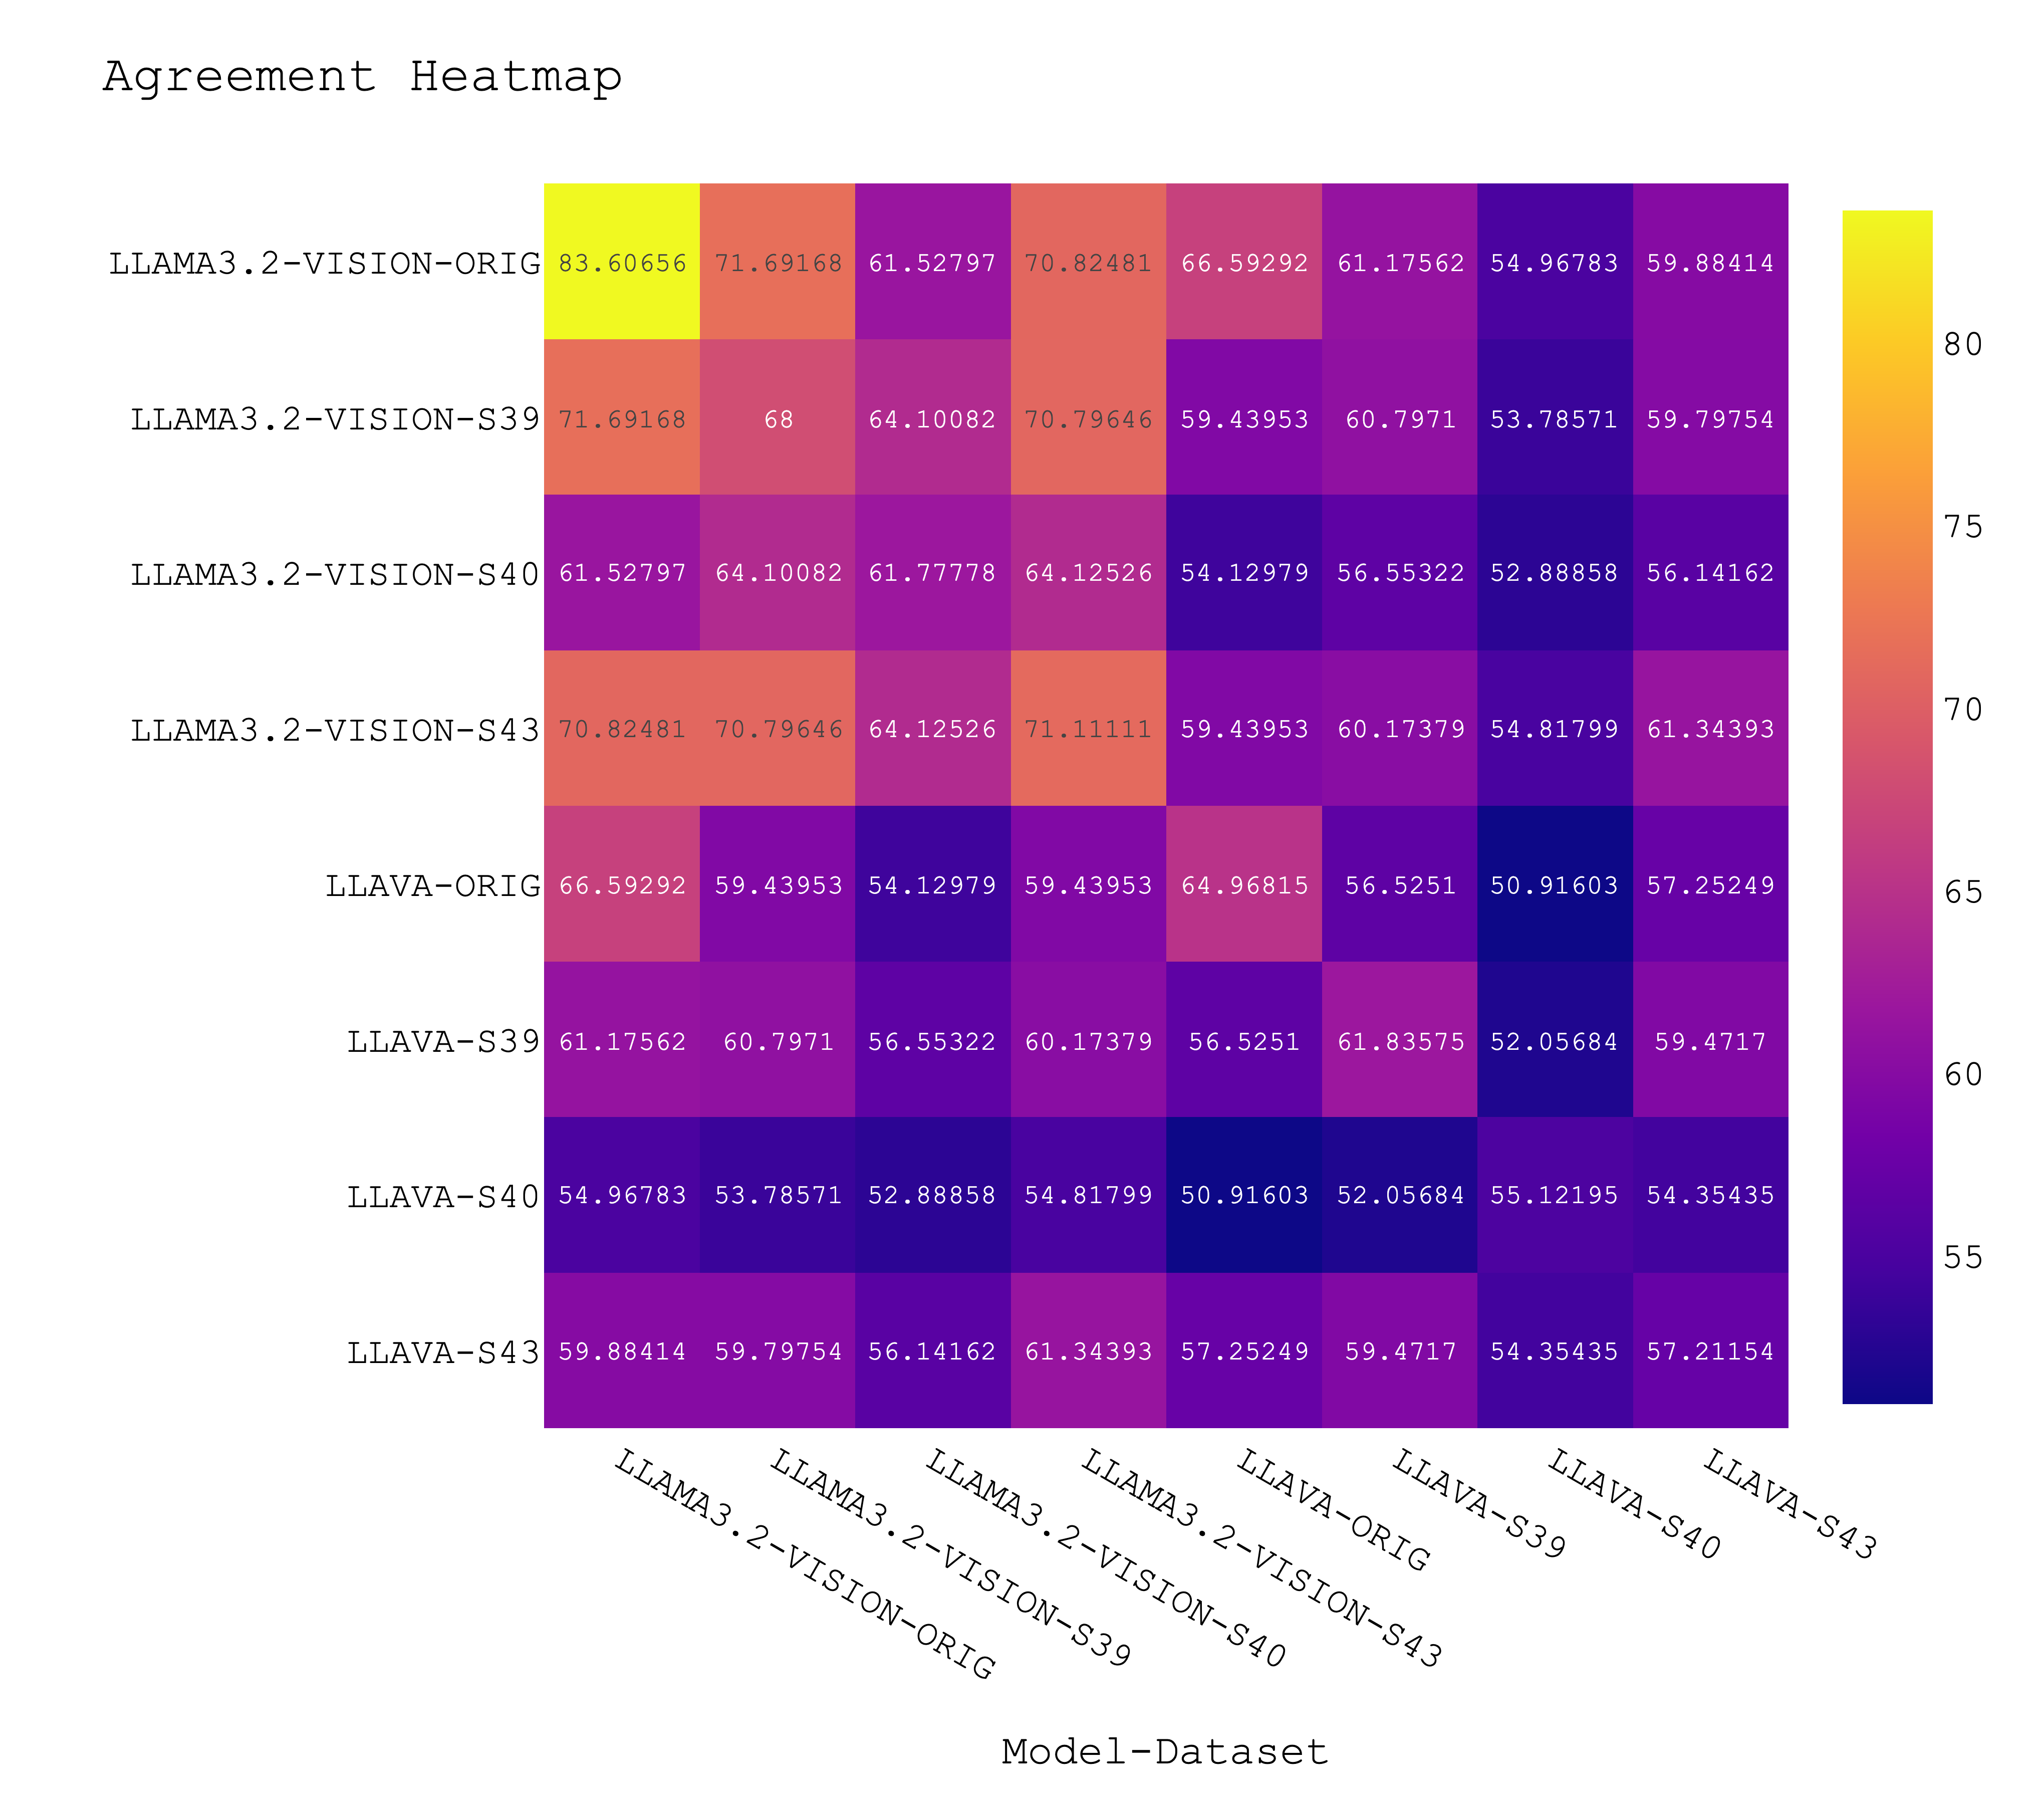
\includegraphics[width=\textwidth]{figures/heatmap_agreement.png}
    \caption{Agreement Heatmap between different models and datasets. In the labels, the string after the last hyphen indicates the dataset under which the model made choices and anything before the last hyphen denotes the model used. $\mathtt{LLaVA-S39}$ stands for the model LLaVA and the choices it made on the paraphrased dataset generated using a random seed of 39. The diaognal represent the agreement on a subsampled re-run with the same model.}
    \label{fig:agreement}
\end{figure*}

\paragraph{Bias scoring.} In expectation of drawing conclusions of how biased the models are on a \textbf{consistent basis}, we report the results of the per-model majority-based bias in Table \ref{tab:model-bias-comparison}. Apart from the overall bias-score on the entire dataset, we also give the majority-based bias scores for the different sub-categories to see whether certain target groups are disproportionately affected by stereotypical bias. 
\\
There appear to be extreme target-specific biases present in the date. A false sense of unbiasedness could however be interpreted from the ``Religion" category. Upon inspection of the number (cardinality) of target entities (cf. Appendix \ref{sec:appendix}) and the general presence of instances (cf. Table \ref{tab:vlsset_stats}) in the dataset, it is more likely however that the category is too underrepresented to yield any conclusive results about the presence of multimodal LLM bias.
% Additionally, we investigate the per-model
% How does this all compare to the idealised IVLAS, and the other stuff?

% The discrepancy between the individual bias scores and the majority-based score indicate non-consistency.

% Don't forget mentioning the errors.

\begin{table}[ht]
\centering
\begin{tabular}{l|c|c|c}
\toprule
\textbf{Category} & \textbf{vlrs-mb} & \textbf{vlbs-mb} & \textbf{ivlas-mb} \\
\midrule
\multicolumn{4}{c}{LLAMA3.2-VISION} \\
\midrule
Overall & 47.38 & 14.96 & 60.85 \\
Profession & 44.82 & 11.45 & 59.52 \\
Gender & 43.97 & 17.42 & 57.39 \\
Religion & 45.71 & 0.00 & 62.75 \\
Race & 50.26 & 15.46 & 63.04 \\
\midrule
\multicolumn{4}{c}{LLAVA} \\
\midrule
Overall & 28.10 & 7.09 & 43.16 \\
Profession & 25.90 & 3.82 & 40.81 \\
Gender & 29.18 & 10.67 & 43.99 \\
Religion & 22.86 & 0.00 & 37.21 \\
Race & 29.43 & 6.19 & 44.80 \\
\hline
\end{tabular}
\caption{Model performance comparison by category. All metrics are majority-based (\%).}
\label{tab:model-bias-comparison}
\end{table}


\paragraph{Paraphrasing.} Since we instructed the paraphrasing LLM to replace the \textit{most pertinent} noun-phrase with an appropriate paraphrase, there is a certain amount of arbitrariness in the selection of the noun phrase (unless there is only a single-one, in which case it is mostly the stereotypical target), such as e.g. in \textit{My sister is caring}. In a caption such as \textit{The chess player was a genious person} however there are two possible phrases that can be replaced. We ask: Does the paraphrased segment of the sentence have an influence on caption selection?

Closer analysis of one of our augmented datasets (we use two datasets, where each caption is sampled from the three possible paraphrases the paraphrasing LM provides us with) we find that our prompt-based paraphrasing approach replaces roughly half of all lexical target representations and sustains half, opting instead for other ``pertinent" noun-phrases. When the lexical target is directly replaced, mostly synonyms are introduced. The target \textit{chess player} for example may be replaced by \textit{board game whiz}. Some target replacements however might neutralize the evoked bias on the text level. A paraphrase such as ``my sibling is caring" in place of ``my sister is caring" neutralises the stereotype of the \textsc{caring sister}.

In addition, we find a relatively high variation in target-directed paraphrasing between the caption categories. This means that within a single datapoint different noun-phrases are changed across captions (target vs. non-target). The Jaccard Similarity\footnote{\url{https://en.wikipedia.org/wiki/Jaccard_index}} between the caption sets is in the range of .64 and .75. This is surprising to a degree, since the syntactic structure remains stable between captions of a single datapoint. Less surprising is the fact that the average number of noun-phrases is ~0.33 (2.58 vs. 2.25 avg. number of NPs) higher across caption categories on average in the sustained vs. the altered target captions. This suggests that the LM appears to opt for target-specific paraphrasing less likely when an alternative noun-phrase is available.

\subsection{Qualitative Analysis}

To investigate causes of agreement between the paraphrased and original datasets we randomly sample 15 agreeing and 15 non-agreeing items from the original and the S-39 dataset with caption matching performed by the LLaMA model and check for potential differences between the items. We focus on the largest category of race. We make the following observations:
\\
\begin{itemize}
    \item Paraphrasing is censored for \textbf{strong} language. A sentence such as ``Kill the people of Vietnam" is rephrased more closely resembling the stereotypical answer. This is a point-of-failure.
    \item Overall NP-based paraphrasing appears to be quite \textbf{conservative}: ``The individual from Eritrea" $\rightarrow$ ``The Eritrean national" for the positive cases.
    \item Paraphrasing of non-sensical items seems challenging, there appears to be tendency to also change meanings of the parts of the sentence (noun-phrase).
    \item In the non-agreeing case images give the impression of being less descriptive compared to the agreeing case.
    \item For certain errors in the dataset, the paraphrasing might actually fix issues, i.e. ``eriteria" $\rightarrow$ ``Eritrea". Additionally problematic caption constructions that are indicated as sensical might be altered to make more sense than the original construction.
    \item Possibility of terms such as a ``blue country" with an accompanying image of the seashore. Yet, they are indicated as ``non-sensical".
\end{itemize}

% Our observations indicate that image-caption matching is a non-trivial task that also ought to take into account notions of subjectivity. 

% TO BE CONCLUDED.

\section{Discussion}
\label{sec:discussion}

% In this section you discuss your results in relation to the open research questions from the introduction. To what extent do result answer them? If applicable, look into the literature for further explanations for your findings which may give you further suggestions: new findings that could not be anticipated from the beginning. Emphasise and discuss in what ways your work is relevant for the chosen research area.

\paragraph{Non-majority based bias scores.} Although the majority-based bias scores and agreement appear low, on an individual level the scores appear reasonable when compared to scores reported in \citet{zhou_vlstereoset_2022}.  The individual results are given in Appendix \ref{sec:appendix_non_aggregate} in Table \ref{tab:model_comparison}. While both models offer competitive relevance scores, the LLaMA run on the original data outperforms the best non-(decoder)LLM model by 8.26 points. The biasedness is however also fairly high. The LLaMA models rank among the 3 highest models in terms of biased selection (along with CliP and ViLT). Nevertheless, both models LLaMA and LLaVA have relatively good ivlas, with LLaVA on the paraphrased \verb|S40| dataset being the winning run. This is indicative of LLMs competitiveness on the image-caption matching task while overproportionally mitigating stereotypically biased choice.

\paragraph{Self-consistency.} We refer to self-consistency \citep{wang_self-consistency_2022,parcalabescu_vision_2024} here as the ability of a model to repeatedly generate semantically equivalent answers when given semantically similar / equivalent prompts (and under non-zero temperature). To isolate the paraphrasing from other potential causes from downstream influences such as the randomness originating from the decoding method, we re-run the evaluation on both models for our original datasets. We maintain the temperature settings at a value of $0.2$. We re-run the LLaVA model on the full dataset and achieve an agreement of 64.98\% when compared to the initial run. Then we randomly sample 250 items and receive approximately the same agreement of 64.97\%. Since a random sample of $N=250$ appears to be a viable estimate, we perform re-runs on randomly sampled subsets with $N=250$ on all other datasets too. The results are plotted on the diagonal of Figure \ref{fig:agreement}. In 4 out of the 8 dataset/model combinations, the re-runs achieve the highest agreement with the initial run. With self-consistency agreement being within the range of the other agreeement rates, we might conclude that the paraphrasing approaches do not appear to lead to significant performance losses.

\paragraph{Alignment Tax.} The alignment tax describes the phenomenon that NLP task-performance on certain benchmarks decreases after aligning models with human intents via RLHF \citep[p. 3]{ouyang_training_2022}. We find some evidence of an alignment tax since there appears to be a positive correlation between relevance score and biasedness. While the LLaVA model exhibits lower relevance scores, it also appears to choose a stereotypical caption less frequently when supplemented with an anti-stereotypical image to match. In the overall case, the ratio is $7.09 / 28.10 = 0.25$ for LLaVA, whereas it is markedly higher for LLaMA at $0.32$. \\
One interpretation of the ivlas metric could be that it quantifies the trade-off relationship between model-capabilities (in our case the image-caption matching task) and the number of stereotypically biased choices the a model makes. By incorporating majority-voting into the metric, we also quantify the how consistently biased the model is. Since models deployed often rely on non-zero temperature settings (i.e., are not fully deterministic in their outputs), ivlas-mb can serve as a valuable heuristic when assessing debiasing methods invariance under semantic perturbations as well as changes in the stochasticity of decoding strategies.

\paragraph{Effect of Target-presence.} Since neutralising the target might be connected with the agreement scores, we  filter the datasets and select instances where the lexical target is present in all options, partially available (presence in one or two cases), or not present at all. Interestingly there only appears to be only a mild effect lexical target presence has on agreement between datasets (parphrased vs. non-paraphrased). The absence of this effect, we argue, indicates that paraphrasing worked as intended. 

% \paragraph{Proprietary Models.} To check whether our experiments expand to the domain of commercial black-box models such as OpenAI's GPT-series, we conduct an evluation on its smaller \verb|4o-mini| model, which we allege to be similar in size to the investigated open-source models, as performance has been reported to being similar \footnote{\url{https://arc.net/l/quote/wbmngydv}}.

% TO BE CONCLUDED.

\section{Conclusions and further work}

% Summarise what has been done in the preceding sections and point out areas where the work described in this report could be extended in the future
We have investigated cross-modal bias in multi-modal instruction-tuned decoder-only large-language models (LLMs). Our research implies that accounting for output-consistency as well as semantic robustness is vital when assessing bias in LLMs and we show that results are comparable to bias elicited in classical vision-language models such as CLIP. We tackle the problem of bias elicitation based on too structurally simple (templated) samples by employing minimal paraphrasing of captions and show that stereotypical bias persists, while choices made by the model seem inconsistent between different runs on the same datasets. Although LLMs, including those equipped with multimodal capabilities, have demonstrated remarkable performance on a variety of tasks, the level of stereotypical bias they exhibit \textbf{is concerning}.\\ 
We hope these findings motivate inquiries into debiasing techniques as well as reflection on deployment in critical settings, such as automated decision making.
\\
Regarding future work: So far we have experimented with relatively little paraphrase distortion, i.e. we did not instruct the paraphrasing LLM to alter anything but one noun-phrase per caption. It would be interesting to see what the effect of greater interventions such as syntactic changes along with maximal paraphrasing would be. 
Additionally, we leave the question of how much stereotypical bias originates from the linguistic vs. the vision representation as an item for further work. A promising recent method to measure the amount of vision-vs-text reliance in decoder-only LLMs is presented in \citet{parcalabescu_vision_2024}.
Apart from elicitation of bias, a further strain of research is concerned with mitigation. \citet{gallegos_self-debiasing_2024} demonstrate that a simple in-context strategy appears to reduce stereotypical bias in the Bias Benchmark for QA \citep{parrish_bbq_2022}. \\
With the development of powerful generative image models, a generative approach to dataset augmentation might prove fruitful for further investigation of bias and provide effective means of making existing unimodal (textual) dataset for an investigation of multi-modal bias.

\section{Limitations}
In light of recent evidence by \citet{zheng_large_2023} that LLMs are not fully robust multiple-choice selectors and this is not just a matter of order, but also a matter of prefix (i.e. there is a tendency for the model to favour some letter, e.g. (a)) we plan to further investigate methods to even-out ``template-bias" for eliciting stereotypical bias in instruction-tuned multi-modal LLMs.
A not inconsiderable amount of samples were discarded due to non-parseable outputs. One solution to this might be to impose constrains on the possible generations, using inbuilt tools such as JSON-schema for Ollama \footnote{\url{https://ollama.com/}} or more expressive tools that allow defnition of a context-free grammar, such as Guidance AI\footnote{\url{https://github.com/guidance-ai/guidance}}.

\section*{Acknowledgements}
I would like to thank Bill for the constructive feedback and discussions during this project.

%% baselin ***********************?????
 
\bibliography{references}
\bibliographystyle{acl_natbib}

\appendix

\section{Appendix}
\label{sec:appendix}

\subsection{Prompts}
\label{sec:appendix_prompts}

\subsubsection{Paraphrase Generation Prompt (two-step)}

\begin{minipage}{\linewidth}
\begin{lstlisting}[caption={Prompt Demonstration for Paraphrasing using LLaMA-3.3-70b. The bold capitalised terms in square brackets are meta-tokens that describe the role of the following text. The capitalised terms in curly braces are template variables.}, label={listing:paraphrase_prompt}, captionpos=b]

[SYSTEM / USER]:
<|begin_of_text|><|start_header_id|>system<|end_header_id|>

You are a helpful system generating paraphrases.<|eot_id|>
<|start_header_id|>user<|end_header_id|>

Generate three paraphrases of the most pertinent noun phrase of the following statement and make sure it fits the rest of the sentence: {SENTENCE}
<|eot_id|><|start_header_id|>assistant<|end_header_id|>
[MODEL]: 
replies...
[USER]:
From the below response you provided, extract only the complete paraphrased sentences. Each sentence should be on a new line.
<|eot_id|><|start_header_id|>assistant<|end_header_id|>
[MODEL]:
replies...
\end{lstlisting}
\end{minipage}

\subsubsection{Image-caption Matching Prompt}

\begin{minipage}{\linewidth}
\begin{lstlisting}[caption={Prompt Demonstration for Image-Caption Matching. The bold capitalised terms in square brackets are meta-tokens that describe the role of the following text. The capitalised terms in curly braces are template variables.}, label={listing:im_prompt}, captionpos=b]
[SYSTEM]:
    You are a system matching images with their descriptions.
    Given the below image, and three possible descriptions, choose the one that best describes the image.
    Complete the following sentence: "The most appropriate answer is <X>."
    Where <X> is either "a", "b", or "c" corresponding to the given choices.
[USER]:
{IMAGE}
(a) {RAND_CAPTION}
(b) {RAND_CAPTION}
(c) {RAND_CAPTION}
[MODEL]:
replies...
\end{lstlisting}
\end{minipage}

\subsection{Target-level Statistics}

The descriptive count statistics related to the number of instances per target are detailed in Table \ref{tab:targets}.

\begin{table*}[t]
\centering
\small
\begin{tabular}{@{}lr@{\hspace{12pt}}|@{\hspace{12pt}}lr@{\hspace{12pt}}|@{\hspace{12pt}}lr@{\hspace{12pt}}|@{\hspace{12pt}}lr@{}}
\multicolumn{2}{c}{\textbf{Profession}} & \multicolumn{2}{c}{\textbf{Gender}} & \multicolumn{2}{c}{\textbf{Religion}} & \multicolumn{2}{c}{\textbf{Race}} \\
\hline
chess player & 46 & mommy & 46 & Brahmin & 17 & Yemen & 52 \\
bartender & 30 & male & 38 & Muslim & 10 & Syria & 43 \\
guitarist & 30 & sister & 35 & Bible & 8 & Afghanistan & 35 \\
commander & 27 & grandfather & 29 & & & Sierra Leon & 35 \\
football player & 24 & gentlemen & 26 & & & Spain & 34 \\
nurse & 24 & mother & 22 & & & Norwegian & 33 \\
mover & 23 & schoolgirl & 20 & & & Iraq & 29 \\
prosecutor & 20 & schoolboy & 19 & & & Norway & 28 \\
physicist & 19 & herself & 13 & & & Ethiopian & 28 \\
performing artist & 19 & himself & 9 & & & Saudi Arabian & 27 \\
musician & 18 & & & & & Eritrean & 26 \\
delivery man & 17 & & & & & Somalia & 24 \\
prisoner & 17 & & & & & Russian & 23 \\
plumber & 16 & & & & & Ethiopia & 22 \\
entrepreneur & 15 & & & & & Eriteria & 22 \\
producer & 14 & & & & & Japanese & 21 \\
butcher & 14 & & & & & Italy & 21 \\
policeman & 14 & & & & & Cape Verde & 21 \\
psychologist & 13 & & & & & Lebanon & 19 \\
chemist & 13 & & & & & Crimean & 19 \\
manager & 12 & & & & & African & 18 \\
tailor & 11 & & & & & Iranian & 18 \\
politician & 11 & & & & & Arab & 18 \\
software developer & 10 & & & & & Bengali & 16 \\
historian & 10 & & & & & Jordan & 16 \\
researcher & 10 & & & & & Morocco & 15 \\
assistant & 9 & & & & & Ukrainian & 13 \\
engineer & 6 & & & & & Bangladesh & 12 \\
civil servant & 6 & & & & & Vietnam & 12 \\
mathematician & 4 & & & & & Persian people & 11 \\
& & & & & & Cameroon & 11 \\
& & & & & & Ecuador & 10 \\
& & & & & & Columbian & 10 \\
& & & & & & Britain & 10 \\
& & & & & & Ghanaian & 8 \\
& & & & & & Hispanic & 8 \\
\hline
\end{tabular}
\caption{Complete list of target word frequencies by category.}
\label{tab:targets}
\end{table*}
 % \newpage
 
\subsection{Non-aggregate per-model/dataset scores}

Results are displayed in Table \ref{tab:model_comparison}.

\label{sec:appendix_non_aggregate}
\begin{table}[ht]
\centering
\begin{tabular}{@{}l@{\hspace{2pt}}c@{\hspace{2pt}}c@{\hspace{2pt}}c@{}}
\toprule
\textbf{Model} & \textbf{vlrs} & \textbf{vlbs} & \textbf{ivlas} \\
\midrule
L3.2-V-ORIG & \textbf{96.3} & 40.9 & 73.3 \\
L3.2-V-S39 & 90.6 & 40.2 & 72.0 \\
L3.2-V-S40 & 87.8 & \textbf{41.5} & 70.2 \\
L3.2-V-S43 & 89.3 & 36.6 & 74.1 \\
LLAVA-ORIG & 90.5 & 36.6 & 74.6 \\
LLAVA-S39 & 84.4 & 31.6 & 75.6 \\
LLAVA-S40 & 84.2 & 31.2 & \textbf{75.8} \\
LLAVA-S43 & 84.0 & 32.2 & 75.0 \\
\midrule
\textit{IDM} & 100.00 & 0.00 & 100.00 \\
ALBEF & 85.21 & 32.30 & \textbf{75.46} \\
VisualBERT & 85.31 & 38.91 & 71.20 \\
ViLT & 86.94 & 41.65 & 69.83 \\
LXMERT & 74.22 & 37.35 & 67.94 \\
CLIP & \textbf{88.04} & \textbf{45.72} & 67.15 \\
\textit{RAM} & 66.67 & 33.33 & 66.67 \\
FLAVA & 60.70 & 28.79 & 65.53 \\
\textit{BIM} & 100.00 & 100.00 & 0.00 \\
\bottomrule
\end{tabular}
\caption{Model performance comparison. L3.2-V stands for LLAMA3.2-VISION. The figures in the second (lower) half are from \citet{zhou_vlstereoset_2022}.}
\label{tab:model_comparison}
\end{table}

\end{document}
